\chapter{Algorithms and Implementation}

\section{Interface Implementation}\label{interface-implementation}

One of the core components of Foldlings is the interface. To create
features, we capture touch input, display a preview of fold features as
the user creates them, and add created features to the fold pattern.
This system is outlined in Figure \ref{mvc}.

\begin{figure}[htbp]
\centering
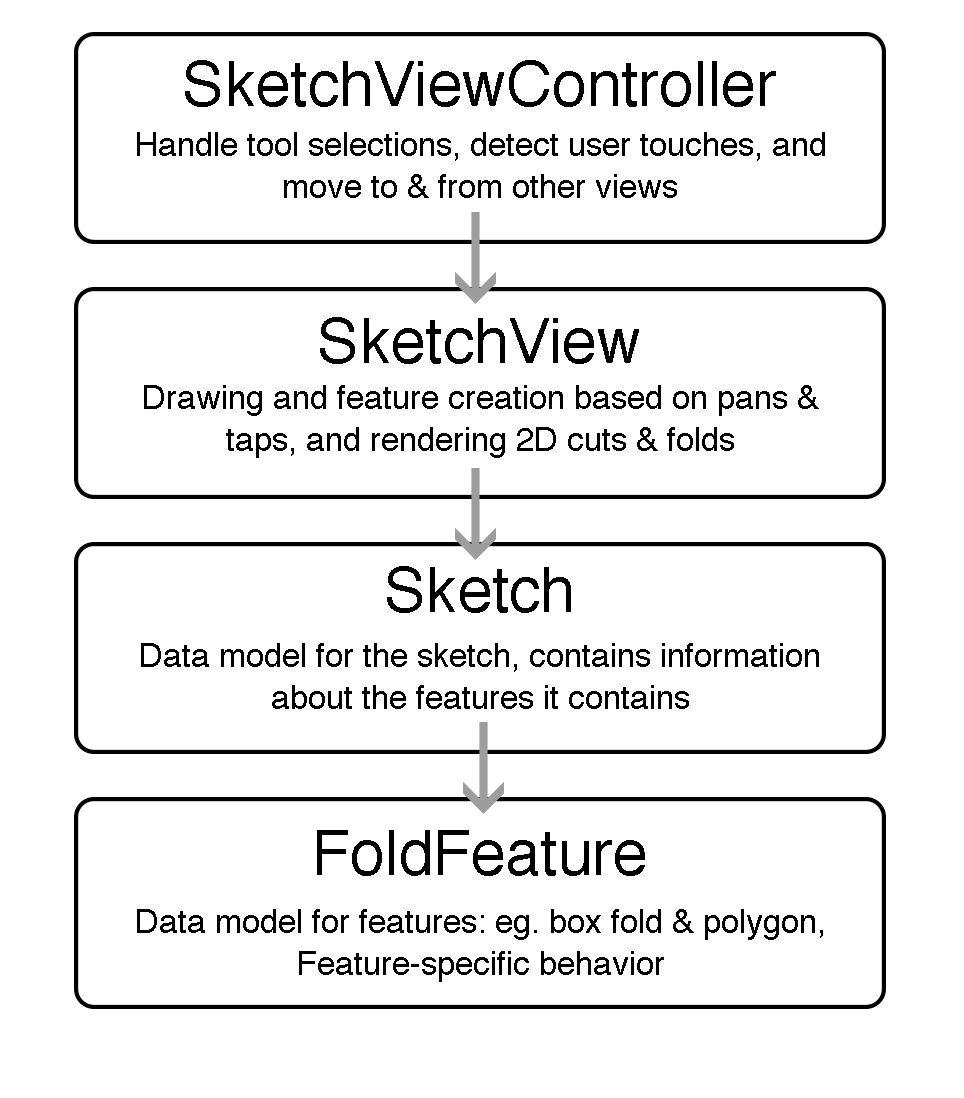
\includegraphics{figures/40_Tech_Interface_Implementation/sketchview-descendents-thesis-figure.png}
\caption{Relationship between interface classes: a SketchViewController
manages a SketchView that contains a Sketch that contains FoldFeatures.
\label{mvc}}
\end{figure}

Although this structure borrows heavily from the Model-View-Controller
design pattern, we do not follow the pattern strictly. The MVC paradigm
often becomes muddy, with much information shared between the separate
modules (\citet{veit2003model}). In our case, we separate modules not
purely based on MVC encapsulation but based on functionality. For
example, rather that strictly separating all touch handling into the
view controller or all drawing into the view, these responsibilities are
shared between the classes as needed to perform their roles. See section
\ref{touch-handling}, below, for more information.

\subsection{Touch Handling}\label{touch-handling}

In order to create features, we first need to capture touch input.
Foldings handles two types of touches: pan gestures, and tap gestures.
Apple describes gesture recognizers in the documentation for the
\emph{UIGestureRecognizer} class:

\begin{quote}
Gesture recognizers convert low-level event handling code into
higher-level actions. They are objects that you attach to a view, which
allows the view to respond to actions the way a control does. Gesture
recognizers interpret touches to determine whether they correspond to a
specific gesture, such as a swipe, pinch, or rotation. If they recognize
their assigned gesture, they send an action message to a target object.
The target object is typically the view's view controller, which
responds to the gesture\ldots{}
\end{quote}

In Foldlings, all gestures are captured by the SketchViewController,
which passes un-handled gestures on to classes lower down the chain. In
general, all taps are handled at the SketchViewController level; the
only exception to this rule is the Polygon feature, described in section
on page. \textbf{\textgreater{}\textgreater{}TODO PAGES}

\subsection{Tool Selection}\label{tool-selection}

Tool state is maintained by the SketchViewController. The
SketchViewController handles taps on tool buttons and features, and
passes pan gestures to the SketchView. The method called on the
SketchView depends on what feature was selected. The function below in
SketchView captures pan gestures, and calls the appropriate function
depending on the tool selected and the drawing state.

\small
\singlespacing 

\begin{pygmented}{swift}
    func handlePan(sender: AnyObject) {
        if(sketch.tappedFeature != nil){
            switch(sketch.tappedFeature!.activeOption!){
            case .MoveFolds:
                handleMoveFoldPan(sender)
            default: break
            }
        }
        else{
            switch (sketchMode) {
            case .BoxFold:
                handleBoxFoldPan(sender)
            case .FreeForm:
                handleFreeFormPan(sender)
            case .VFold:
                handleVFoldPan(sender)
            case .Polygon:
                handlePolygonPan(sender)
            default:
                break
            }
        }
    }
\end{pygmented}

\doublespacing
\normalsize

Within the specific function in SketchView, pan gestures are converted
into feature edges by listening to \emph{touchesBegan},
\emph{touchesMoved}, and \emph{touchesEnded}. When a pan begins, we
create a new feature of the appropriate type and set it as the currently
active drawing feature. When the pan is updated, we add and/or modify
edges in the active feature. When the pan ends, we make final
modifications to edges, validate the feature, and add it to the sketch.

\textbf{\textgreater{}\textgreater{}TODO, COULD ADD ALGO HERE}

Of course, the implementation of pan delegate methods varies widely
between features. For example, a diagonal pan with the box fold tool
selected would create folds and cuts to form a box between the start and
end point, whereas the same touch in the freeform tool would create

\subsection{Fold Feature Preview}\label{fold-feature-preview}

While the user is drawing, the SketchView displays a preview of the
feature in progress, to give feedback on the drawing. Meanwhile, the
SketchView also displays the previously drawn features that have been
added to the sketch. Although the display of cuts and folds for the
current feature is visually similar to those of the final feature, the
method of drawing a preview version of the currently active feature
varies from the generation of final feature edges.

We store the currently active feature separately, it is not added to the
list of features until it is completed and passes validation. Thus, its
edges are drawn by the function that draws all edges currently in the
sketch. For performance reasons, we display a preview of the active
feature on top of all features in the sketch --- modifications to
existing features, and expensive operations such as truncation for
freeform shapes, are performed only when the feature is added to the
sketch. During drawing, we display the set of preview edges stored in
the feature, which sometimes differ from the final feature edges.

For box folds, we display a preview of all the edges, but do not occlude
the middle fold until the feature is completed. For freeform features,
we do not perform truncation until the feature is completed (and spans a
driving fold). As a preview, the SketchView shows the user's touch path
as a cut. For polygons, we display control circles at vertices. These
circles indicate that the vertices are draggable, modifying edge
endpoints dynamically. For v-folds, we display a dynamic preview of the
vertical cut and top and bottom diagonal folds. The middle diagonal
angle is not calculated until the feature is added to the sketch.

\subsection{Feature Creation}\label{feature-creation}

Once the user completes a feature, we add it to the sketch\footnote{Assuming
  the feature is valid. See section on page
  \textbf{\textgreater{}\textgreater{}TODO: cite validity}}. Adding a
feature to the sketch requires modifying existing features in the
sketch, constructing parent-child relationships, and recalculating
planes from edges. How these tasks are achieved depends on the specific
FoldFeature class.

The specific implementations of the FoldFeature superclass are described
in Chapter \ref{tool-implementation} on page
\pageref{tool-implementation}. The Sketch class contains methods for
adding and removing features from the sketch. It also contains
lower-level functions for adding, removing, and replacing edges. These
methods are typically called by feature-specific methods that modify the
sketch, such as \emph{splitFoldByOcclusion}.

In addition to adding a feature to the sketch, we also calculate the
planes, as described in \textbf{\textgreater{}\textgreater{}MARISSA}.
This allows us to shade planes based on orientation. After calculating
planes from edges, relationships between planes are stored in the plane
tree within the sketch. Within \emph{getPlanes}, plane orientations are
set by traversing the plane tree, alternating between vertical and
horizontal.

\subsection{Hierarchy}\label{hierarchy}

A key aspect of blah blah blah is hierarchy

Features contain other features

both feature and plane hierarchy
